\documentclass[journal]{IEEEtran}
%\IEEEoverridecommandlockouts
% The preceding line is only needed to identify funding in the first footnote. If that is unneeded, please comment it out.

% listings package for code blocks
\usepackage{listings}
\usepackage{xcolor}
\usepackage{cite}
\usepackage{verbatim}
\usepackage{graphicx}
\usepackage{parskip}

\begin{document}

% overfull \hbox .. too wide 
\setlength{\emergencystretch}{12pt}
%\setlength{\parskip}{0pt} % 1ex plus 0.5ex minus 0.2ex}
\setlength{\parindent}{10pt}

\definecolor{codegreen}{rgb}{0,0.6,0}
\definecolor{codegray}{rgb}{0.5,0.5,0.5}
\definecolor{codepurple}{rgb}{0.58,0,0.82}
\definecolor{backcolour}{rgb}{0.95,0.95,0.92}

\lstdefinestyle{mystyle}{
    backgroundcolor=\color{backcolour},   
    commentstyle=\color{codegreen},
    keywordstyle=\color{magenta},
    numberstyle=\tiny\color{codegray},
    stringstyle=\color{codepurple},
    basicstyle=\ttfamily,
    breakatwhitespace=false,         
    breaklines=true,      
    postbreak=\mbox{\textcolor{red}{$\hookrightarrow$}\space},           
    captionpos=b,
}

\lstset{style=mystyle}

\title{Ranking Classification Models using Receiver Operating Characteristics}

\author{
\IEEEauthorblockN{Lillian Mueller}
\IEEEauthorblockA{lmuelle1@umd.edu}
}

\maketitle

\begin{abstract}
\label{log:abstract}

ROC, or receiver operating characteristics, are used to rank the performance of classification models. Using this method, this investigation examines what model is better at predicting whether a flight may be delayed or not. The models examined are a decision tree classification model and a logistic regression model. After training these models on a flight dataset taken from the American Statistical Association (ASA) Statistical Computing Dataverse, the logistic regression model proved to have slightly better performance than the decision tree model based on the AUC, or area under the curve, calculation derived from the models' respective ROC curve. Understanding the dataset and the model, including its flaws, is essential to determining the best fit evaluation method to evaluate it. 

\end{abstract}

\section{Introduction}
\label{sec:intro}

Being able to evaluate and rank classification models is just as important as developing them. If an analyst cannot properly evaluate a model and compare it to another, the analyst may never be able to find a well-fitted model for the dataset. Using a dataset of flight data, the methods for the evaluation of classification model ranking measurements can be tested to determine the best model for predicting whether or not a flight will be delayed. The method of choice is the creation of Receiver Operating Characteristics Curves, or ROC curves, for each model. These curves show the model's performance graphically by displaying the model's true positive rate versus the model's false positive rate, effectively the trade-offs between benefits and costs made by the model \cite{b1}. 

Regarding the flight dataset, this dataset is taken from the American Statistical Association (ASA) Statistical Computing Dataverse and the data associated with 2008 is used in this investigation \cite{b2}. Attributes from this collection include date and time of the flight, aircraft carrier and unique identification numbers, airport of origin and destination, distance of flight, and various delay times based on cause. By condensing the delay times into a classification target set, the models are developed to classify whether the flight will be delayed or not. 

Section \ref{sec:methodology} describes how to use Python to clean the data, develop the models, and compare the models' performance. The final determination of the best fit model is in Section \ref{sec:results}. Finally, the results and future research is discussed in Section \ref{sec:discussion}. 

\section{Methodology}
\label{sec:methodology}

This investigation entails using various classes from the library \lstinline{scikitlearn}. To develop the models: the \lstinline{DecisionTreeClassifier} class from the \lstinline{tree} module and the \lstinline{LogisticRegression} class from the \lstinline{linear_model} module were used. To develop the accuracy/precision scores, Receiving Operator Characteristic curves, and associated metrics of each model ,  \lstinline{sklearn}'s \lstinline{metrics} module was used. Other Python libraries were used along the was as well to help handle the data which includes \lstinline{matplotlib.pyplot}, \lstinline{pandas}, \lstinline{math}, and \lstinline{numpy}. 

\subsection{Cleaning the Dataset}

After downloading the dataset, the file corresponding to 2008 was chosen. In order to read this file, the \lstinline{read_csv} function from the \lstinline{pandas} library was used. This function requires the name of the file being read and as the file was compressed, the compression type, “bz2” was also specified. This created a DataFrame of the data contained within the file. Since the raw file contained many more fields than necessary, the extra columns were dropped from the DataFrame using \lstinline{df.drop(columns=[])}. Columns dropped included 'Year', 'FlightNum', 'TailNum', 'Distance', and 'AirTime', just to name a few. The remaining columns included 'Month', 'DayOfWeek', 'DepTime', 'UniqueCarrier', 'Origin', 'Dest', 'CarrierDelay', 'WeatherDelay', 'NASDelay', 'SecurityDelay', and 'LateAircraftDelay'.

Upon reviewing the remaining columns, many of the columns pertaining to the delay contained “nan”, which means there was a gap in the data. In this dataset, each delay column pertains to the minutes delayed due to a specific reason, such as weather or security. This means that each “not a number” represented no delay. Therefore, the “nan”, or “not a number”, was replaced with zeros using the \lstinline{.fillna(0)} in each delay column. To make sure there were not any more missing data entries, \lstinline{.dropna()} dropped all other rows that had missing data. To find the total delay for each flight, another column was created, 'TotalDelay', which added each delay column together. The delay columns were dropped afterwards. Finally, to create the target classifications, if the total delay was equal to 0, those flights were coded 0, meaning there was no delay. If the total delay was greater than 0, those flights were coded 1, meaning there was a delay. This split the data about 5:2. 

Regarding the other columns, each needed a bit of work. The month and day of the week column was correctly coded, 1-12 for each month, and 1-7 for each day of the week. Departure time was altered to represent the hour in which the flight departed. The unique carrier column contained the name of the carrier of each flight. Using the carrier information provided with the dataset, each carrier was replaced with its index in the carrier information file. The airport of origin and destination were further filtered. To simplify the dataset, the dataset removed any entries where the flight did not originate from DCA, BWI, or IAD or whose destination was not EWR, JFK, or LGA. Afterwards, once these three airports were left in the respective columns, I coded each 0, 1, and 2 respectively for each column. 

Once the cleaning as finished, I was left with 7379 data points in the dataset. 

\subsection{Creating and Comparing the Models}

For these classification models, the target was the delayed data: did the flight get delayed? The rest of the DataFrame was used as features: the month, day of the week, departure time, carrier, airport of origin, and airport of destination. Once the target array and predictor matrices were determined, the dataset was split into a training and testing set where the testing dataset was 33\% of the data. These sets were then used to train and test the decision tree and logistic regression models. 

For the decision tree model, the methodology of developing this model was similar to that of a previous study \cite{b3}. Specifically for this model, entropy was used as an impurity metric. Additionally, due to the great number of features relative to the Iris dataset, the complexity was decreased by constraining the maximum depth of the tree. Again, the tree was developed using \lstinline{sklearn}'s \lstinline{tree.DecisionTreeClassifier} class. For the logistic regression model, the development of the model mirrored the methodology in another previous study \cite{b4}. The model also did not utilize a penalty term and was developed using the \lstinline{linear_model.LogisticRegression} class. 

In order to compare the performance of the models, the receiver operating characteristics were found for each model in addition to the accuracy scores. The first step was to find the true positive rates and the false positive rates. These rates are derived from confusion matrices and then graphed against each other to form the ROC curve. For each model, \lstinline{SKLearn}'s \lstinline{metrics.roc_curve()} method was used to find the rates, the parameters required for this method include the true classifications and the predicted classifications. A summarizing statistic from this curve was also calculated: the Area Under the Curve, or AUC. This metric was calculated again using the true and false positive rates inputted into the \lstinline{metrics.auc()} method. Using \lstinline{matplotlib.pyplot}, the characteristics from both models were graphed and displayed. 

Finally, as another method to evaluate the performance of the models, cross validation was used to determine the average accuracy. 10 folds were used for this data and the methodology is explained in a previous study \cite{b5}. 

\vspace{50px}

\section{Results}
\label{sec:results}

According to the ROC curves, these models display very poor performance for predicting whether a flight will be delayed. Figure \ref{fig:roc} shows the curve comparison. 

\begin{figure}[h!]
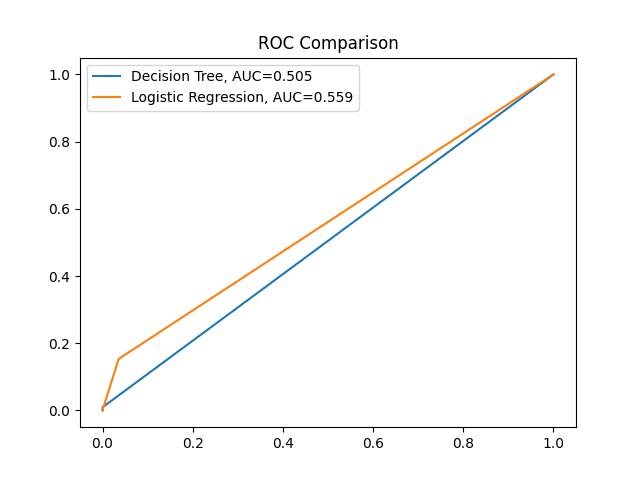
\includegraphics[scale=0.5]{rocCurves.png}
\centering
\caption{ROC Curve Comparison}
\label{fig:roc}
\end{figure}

The area under the curve, or AUC, corresponding to the decision tree model was .505 and the AUC corresponding to the logistic regression model was .559. While this indicated that the logistic regression model is slightly better than the decision tree model, both AUC values are indicative of a bad model. 

After further investigation of the model's performance via cross validation, the following table shows the average accuracy and standard deviations of both models. 

\begin{table}[h!]
\centering
\begin{tabular}{ c | c c }
& Decision Tree & Logistic Regression\\ 
\hline
Mean &	0.680720 &	0.697252 \\
Stardard Dev. &	0.042244 &	0.023287 \\
\end{tabular}
\caption{Model Accuracy Using k=10 Cross Validation}
\label{table:crossVal}
\end{table}

This validates that the logistic regression model is slightly more accurate than the decision tree model. 

\section{Discussion}
\label{sec:discussion}

The results of this investigation were disappointing. Upon creating the receiver operating characteristics curves for each model, the area under the curve, or AUC, for both models were less than .6. This was not expected as there were a lot of data entries and intuitively, there is a trend between the flight time, such as morning versus evening, and a flight being delayed. AUC can be a value in the interval 0 to 1, .5 can be described as a model being as accurate as flipping a coin. An AUC of .5 means the model is unreliable which can be said for the models developed for predicting the flight delays. 

In general, ROC graphs are independent of class proportions and decouple classifier performance from its use case \cite{b1}. This creates a more unbiased evaluation of the model's performance compared to calculating the expected profit using confusion matrices. Since cost and benefit for this classification would be difficult to determine, evaluating the performance using the ROC curves would be more precise. Additionally, the proportion of the classifications in the flight dataset was also very uneven; around 70\% of the data indicated no delay. It is important to not only find a model that best fits the dataset, but also to use an evaluation method that meets the objective of the problem. 

In the future, further modifying the dataset to be more balanced could help with the performance of the model. Since the model was so bias towards one classification, the model was unable to collect enough information about the other class to make accurate predictions about it. Other models may be used in the future as well to compare against the decision tree and logistic regression models. It was clear these models did not portray the data well, perhaps another method would be better.

\begin{thebibliography}{00}
\bibitem{b1}{F. Provost and T. Fawcett, Data Science for Business: What You Need to Know About Data Mining and Data Analytic Thinking, First edition (2005).}
\bibitem{b2}{“Data Expo 2009: Airline on time data.” Harvard Dataverse, Oct. 06, 2008. doi: 10.7910/DVN/HG7NV7.}
\bibitem{b3}
{L. Mueller and R. Hong, “Investigating Decision Trees”.}
\bibitem{b4}
{L. Mueller and R. Hong, “Iris Classification Using Logistic Regression”.}
\bibitem{b5}
{L. Mueller and R. Hong, “Using K-Fold Cross Validation on Decision Tree and Logistic Regression Models to Classify Iris Species”.}

\end{thebibliography}

\end{document}